\documentclass[10pt, a5paper]{article}
\usepackage{pdfpages}
\usepackage{parallel}
\usepackage[T2A]{fontenc}
\usepackage{ucs}
\usepackage[utf8x]{inputenc}
\usepackage[polish,english,russian]{babel}
\usepackage{hyperref}
\usepackage{rotating}
\usepackage[inner=2cm,top=1.8cm,outer=2cm,bottom=2.3cm,nohead]{geometry}
\usepackage{listings}
\usepackage{graphicx}
\usepackage{wrapfig}
\usepackage{longtable}
\usepackage{indentfirst}
\usepackage{array}
\newcolumntype{P}[1]{>{\raggedright\arraybackslash}p{#1}}
\frenchspacing
\usepackage{fixltx2e} %text sub- and superscripts
\usepackage{icomma} % коскі ў матэматычным рэжыме
\PreloadUnicodePage{4}

\newcommand{\longpage}{\enlargethispage{\baselineskip}}
\newcommand{\shortpage}{\enlargethispage{-\baselineskip}}

\def\switchlang#1{\expandafter\csname switchlang#1\endcsname}
\def\switchlangbe{
\let\saverefname=\refname%
\def\refname{Літаратура}%
\def\figurename{Іл.}%
}
\def\switchlangen{
\let\saverefname=\refname%
\def\refname{References}%
\def\figurename{Fig.}%
}
\def\switchlangru{
\let\saverefname=\refname%
\let\savefigurename=\figurename%
\def\refname{Литература}%
\def\figurename{Рис.}%
}

\hyphenation{admi-ni-stra-tive}
\hyphenation{ex-pe-ri-ence}
\hyphenation{fle-xi-bi-li-ty}
\hyphenation{Py-thon}
\hyphenation{ma-the-ma-ti-cal}
\hyphenation{re-ported}
\hyphenation{imp-le-menta-tions}
\hyphenation{pro-vides}
\hyphenation{en-gi-neering}
\hyphenation{com-pa-ti-bi-li-ty}
\hyphenation{im-pos-sible}
\hyphenation{desk-top}
\hyphenation{elec-tro-nic}
\hyphenation{com-pa-ny}
\hyphenation{de-ve-lop-ment}
\hyphenation{de-ve-loping}
\hyphenation{de-ve-lop}
\hyphenation{da-ta-ba-se}
\hyphenation{plat-forms}
\hyphenation{or-ga-ni-za-tion}
\hyphenation{pro-gramming}
\hyphenation{in-stru-ments}
\hyphenation{Li-nux}
\hyphenation{sour-ce}
\hyphenation{en-vi-ron-ment}
\hyphenation{Te-le-pathy}
\hyphenation{Li-nux-ov-ka}
\hyphenation{Open-BSD}
\hyphenation{Free-BSD}
\hyphenation{men-ti-on-ed}
\hyphenation{app-li-ca-tion}

\def\progref!#1!{\texttt{#1}}
\renewcommand{\arraystretch}{2} %Іначай формулы ў матрыцы зліпаюцца з лініямі
\usepackage{array}

\def\interview #1 (#2), #3, #4, #5\par{

\section[#1, #3, #4]{#1 -- #3, #4}
\def\qname{LVEE}
\def\aname{#1}
\def\q ##1\par{{\noindent \bf \qname: ##1 }\par}
\def\a{{\noindent \bf \aname: } \def\qname{L}\def\aname{#2}}
}

\def\interview* #1 (#2), #3, #4, #5\par{

\section*{#1\\{\small\rm #3, #4. #5}}

\def\qname{LVEE}
\def\aname{#1}
\def\q ##1\par{{\noindent \bf \qname: ##1 }\par}
\def\a{{\noindent \bf \aname: } \def\qname{L}\def\aname{#2}}
}


\begin{document}

\title{Базовая серверная архитектура для высоконагруженного стартапа}

\author{Михаил Пянко\\
\small Минск, ООО Анакреон,\texttt{mihail.pianko@warecorp.com}
}
\maketitle

\begin{abstract}
This article describes how to create a good environment for start-up project: what kind of server do we need for each role, and how these servers should communicate. Architecture restrictions are considered. Technical and architecture suggestions are made.
\end{abstract}

На начальном этапе разработки стартапа многие разработчики сталкиваются с проблемой создания достаточно гибкой и в будущем масштабируемой архитектуры приложения, оптимизированной для большой нагрузки. Мы хотели бы поделиться опытом в этой области. В качестве примера рассмотрим методы построения ресурса, базирующегося на Ruby On Rails. Тем не менее примеры, которые будут приведены ниже, с легкостью могут быть использованы для LAMP-решений. 

\section*{Серверы можно разделить на несколько типов по ролям:}
\begin{itemize}
\item Application
\item Database 
\item Load Balancer
\item Utils
\item Tools
\end{itemize}

{\bf Application} --- это frontend-сервер. Возможно использование как одного, так и нескольких Application-серверов. В случае использования одного Application-сервера надобности в балансировке нагрузки нет.

Application сервер выполняет следующие функции:
\begin{itemize}
\item обработка запросов от пользователей (получает запросы от балансировщика нагрузки),
\item взаимодействие с базой данных (Database server),
\item отправка сообщений в очередь сообщений (Utils server),
\item взаимодействие с CDN,
\item взаимодействие с search engines (Util server),
\item инвалидация кэша,
\item работа с кэшем (Database server).
\end{itemize}

Application сервер не должен производить следующих действий:
\begin{itemize}
\item преобразование медиа контента (видео, аудио, слайдшоу, и т.д.),
\item преобразование/кропинг картинок (если позволяет архитектура),
\item отправка сообщений электронной почты (если позволяет архитектура),
\item запросы на сторонние ресурсы через RestClient, curl, etc. (если позволяет архитектура).
\end{itemize}
{\bf Database} --- сервер, на котором находится база данных. В некоторых случаях на Database-сервер также устанавливается memcached, но это зависит от загрузки и конфигурации Database-сервера. 

Database-сервер выполняет следующие функции:
\begin{itemize}
\item обработка запросов от Application и Utils серверов,
\item хранение кэша (в случае установки memcached на DB сервер).
\end{itemize}
{\bf Load Balancer} --- балансировщик нагрузки, необходимый для распределения запросов пользователей между Application-серверами. Простейшим решением является использование nginx в качестве балансировщика нагрузки.

Load Balancer выполняет следующие функции:
\begin{itemize}
\item распределение запросов между Application серверами,
\item обработка HTTPS соединений (SSL сертификат должен быть сконфигурирован на балансировщике),
\item кэширование при использовании Varnish или связки nginx + memcache,
\item Firewall.
\end{itemize}

{\bf Utils} --- сервер, на котором располагаются сопутствующие сервисы, необходимые для отложенной обработки данных. Вот краткий список:
\begin{itemize}
\item message queue (RabbitMQ, Apache Message Queue, etc),
\item search engines (Solr, Sphinx, etc),
\item обработчики сообщений,
\item сервисы для обработки Video, Audio, SlideShow,
\item отправка сообщений электронной почты,
\item взаимодействие с CDN,
\item инвалидация кэша,
\item взаимодействие со сторонними ресурсами (PDF converters, \linebreak SendGrid, etc.). 
\end{itemize}
{\bf Tools} "--- сервер, необходимый для установки сторонних решений для работы приложения. В частности, приложения, базирующиеся на Java/Tomcat, система мониторинга и ресурсы, в безопасности которых вы сомневаетесь (Spellchecker, etc.). Tools-сервер не может установить соединения с Application, Database, Utils-серверами. Единственный протокол взаимодействия "--- это HTTP. Это дает гарантию того, что в результате взлома стороннего компонента основная ферма не пострадает. Сервер с этой ролью не обязателен. 


\begin{figure}[ht]
\centering{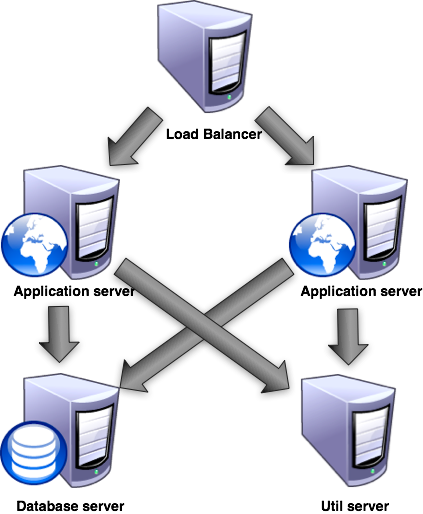
\includegraphics[width=8cm]{09_pianko.png}}
\label{pic:fl1}
%\caption{~}
\end{figure}

\section*{Ограничения, которые накладываются на архитектуру приложения}

\subsection*{Хранение кэша}
Необходимо организовать централизованное хранилище кэша. Файловый кэш и кэширование данных в памяти сервера работать не будет, так как кэш может создаваться и инвалидироваться с разных серверов. Наилучшим решением в данном случае является использования memcached. 

\subsection*{Хранение сессий пользователя}
В данном случае целесообразно хранить сессии в memcached или в Cookies. Отдача сессии на сторону пользователя --- менее безопасное и более медленное решение, чем хранение в memcached. 

\subsection*{Хранение медиа-данных пользователя}
Любой контент, загруженный пользователем на сервер, не может быть просто  сохранен в папку /public/upload. Наилучшим способом хранения данных является CDN. 

\subsection*{Рекомендации по автоматизированной конфигурации серверов}
Существует достаточно большое количество ПО для поддержания конфигурации серверов: Сfengine, Puppet, Chef, Sprinkle. 

Для автоматизированного конфигурирования серверов мы используем Sprinkle. Sprinkle --- это достаточно простое приложение на RoR, позволяющее разрабатывать сценарии по установке ПО на UNIX"=сервера.  Sprinkle поддерживает разделение серверов на роли, фермы и т.д. Так же поддерживаются различные типы инсталяторов, методов проверки текущей конфигурации, источников данных. Sprinkle имеет открытый исходный код, что позволяет вносить изменения в логику работы отдельных компонентов или создавать дополнительные модули. 

\section*{Варианты инсталляции}
Существует несколько вариантов ферм.
\begin{itemize}
\item Single server installation.
  \begin{itemize}
  \item На одном сервере располагаются Application + Util + Database
  \end{itemize}
\item Light farm
  \begin{itemize}
  \item $1$ сервер: Application 
  \item $1$ сервер: Util + DB
  \end{itemize}
\item Big farm:
  \begin{itemize}
  \item $1$ сервер: Load Ballancer 
  \item $x$ серверов: Application
  \item $1-x$ серверов: Util 
  \item $1-x$ серверов: Database (о репликациях и масштабировании базы данных можем поговорить чуть позже) 
  \end{itemize}
\end{itemize}
На самом деле существует множество комбинаций распределения ролей по физическим серверам. Необходимо выбирать оптимальный вариант в зависимости от нагрузки на сервера каждой роли. 

\section*{Рекомендации по архитектуре. Несколько примеров}

\subsection*{Интеграция со сторонними ресурсами}
Зачастую необходима интеграция со сторонними ресурсами для преобразования видео и аудио, обработки слайд-шоу, отсылки писем и т.д. 

Это подразумевает установку соединения по протоколам TCP, HTTP, etc. 
В данном случае существует несколько рисков:
\begin{itemize}
\item сервер недоступен
\item сервер перегружен 
\end{itemize}

В первом случае пользователь не сможет завершить действие, часть данных может быть потеряна или пользователь увидит сообщение ошибки на экране. 
Во втором случае мы получим очень долгую обработку страницы, что доставит неудобство пользователю. 

Лучшим решением в данном случае является отправка события в очередь сообщений и обработка на стороне util"=сервера. 

\subsection*{Обработка картинок пользователя}
Если ваш ресурс поддерживает возможность загрузки аватаров пользователей, логотипов с последующим ресайзингом изображений, вы можете столкнуться с проблемой большой нагрузки на сервер. 

Есть несколько распространенных методов ресайзинга изображений:

\begin{itemize}
\item оригинальное изображение сохраняется в хранилище без обработки. Доступ к изображению со страниц сайта реализован через врапер с элементарной логикой. Если картинка сгенерирована, то необходимо отдать ее через STDOUT или вернуть редирект на статический. Если картинка отсутствует, то сгенерировать и выполнить предыдущий шаг. Проблема этого метода в том, что нагрузка, которую может создать данный алгоритм, не может быть спрогнозирована.  При добавлении нового размера изображения достаточно визита поискового бота - и скорее всего сервера будут перегружены. 
\item оригинальное изображение преобразуется в нужные форматы и размеры непосредственно после загрузки на сервер. Это дает единовременную нагрузку на Application-сервера. Минусом данного метода является задержка в возврате страницы пользователю, что может вызвать дискомфорт.
\item последний вариант является модифицированной версией \linebreak предыдущего. Вместо непосредственной обработки изображения на Application-сервере необходимо отправить событие в очередь сообщения и произвести обработку изображения на Util"=сервере. 
\end{itemize}

\section*{Заключение}

Выше приведены приемы для построения начальной архитектуры высоконагруженной системы, которая в будущем может быть легко расширена и  смасштабирована. Способы дальнейшего развития напрямую зависят от архитектуры приложения, нагрузки на отдельные узлы системы и специфики проекта.

\end{document}




